\competentie
{% competentieformulier
	\competentieformulier
	{% toelichting
		Je bent sensitief, toegankelijk en overtuigend in je
		communicatie met uiteenlopende doelgroepen,
		waaronder klanten. Je neemt de vraag van de klant als
		uitgangspunt, maakt duidelijke afspraken en checkt of
		steeds aan de verwachtingen is voldaan.
	}
	{% deelcompetenties
		Communiceren,
		Rapporteren,%
		Klantgerichtheid%
	}
	{%
		Proof
	}
	{%
		Klantgerichtheid
	}
	{% verwijzing naar bewijs
		\ref{fig:emailclient}
	}
}
{% bewijzen
	\bewijs
	{% naam
		communication with client to achieve best possible product.
	}
	{% starr
		\starr
		{% betreft

			Klantgerichtheid
		}
		{% datum
			20-05-2022
		}
		{% situatie
			Ik ben benaderd door vaccinatiepunt om een web applicatie voor ze te maken.
			De werkgever(vaccinatiepunt) gaf aan moeite te hebben met het inventariseren van de producten.

			De producten liggen op verschillende locaties en hebben allemaal een houdbaarheid datum.
			Doordat de producten nu niet bijgehouden worden op welke locatie en welke houdbaarheid de producten hebben is er een grote kans dat vaccinaties verlopen.



		}
		{% taak
			Een oplossing bedenken die geschikt is voor de huidige sitautie van vaccinatiepunt.
			Door goed naar de wensen van de werkgever te luisteren en hun huidige vaccinatie procedure te bestuderen een applicatie te maken die goed aansluit op het huidige process.

		}
		{% activiteiten
			Ik heb met een werkgever van vaccinatiepunt telefonisch contact gehad.
			Hierbij heb ik aandachtig vragen gesteld over de huidige werk wijzen.

			Ook gaf ik extra veel aandacht aan de door hun beschreven wensen.
			Een makkelijk process waarbij minimale interactie met de applicatie nodig is zodat de aandacht bij de klant is en niet bij het gebruik van de applicatie.

			Met deze informatie ben ik een prototype gaan maken.
			Het prototype moet nog verder getest worden en aangepast worden als de werkgever dit wenst.
		}
		{% resultaat
			Door aandachtig naar de klant te luisteren en met hun huidige process in gedachten heb ik een applicatie gemaakt die goed aansluit bij hun huidige werkwijze.

			Het product is wordt nu getest door de medewerkers en hier uit zullen verdere verbeterings punten naar boven komen.
			Als ik de feedback van de klant krijg zal ik dit implementeren en weer checken bij de klant om zo tot het best mogelijke eindproduct te komen.

			De klant is tot nu toe erg tevrede met het resultaat en door goede communitie en transpirantie is er een uitstekende werknemer/gever relatie.
		}
		{% reflectie
			Ik ben tevreden over de communicatie tussen mij en de werkgever.
			Door aandachtig te luisteren en een goed beeld te krijgen van hun huidige werkwijzen heb ik een goed prototype gemaakt.

			Door te luisteren naar de klant zijn wensen heb ik de wensen weten om te zetten in een techische oplossing die geschikt is voor de klant.

			Ik heb in het verleden ook oplossing gemaakt zonder een goed beeld te hebben van de wensen van de klant.
			Dit eindigde vaak in een applicatie die niet geschikt was voor het werkwijze process.
			Door te veel complexiteit kon de klant de applicatie niet gebruiken.

			Dit is gelukkig nu niet gebeurd.
		}
		{
			Hille: Hille@vaccinatiepunt.nl
		}
	}
	{% bewijs

		\begin{figure}
			\begin{center}
				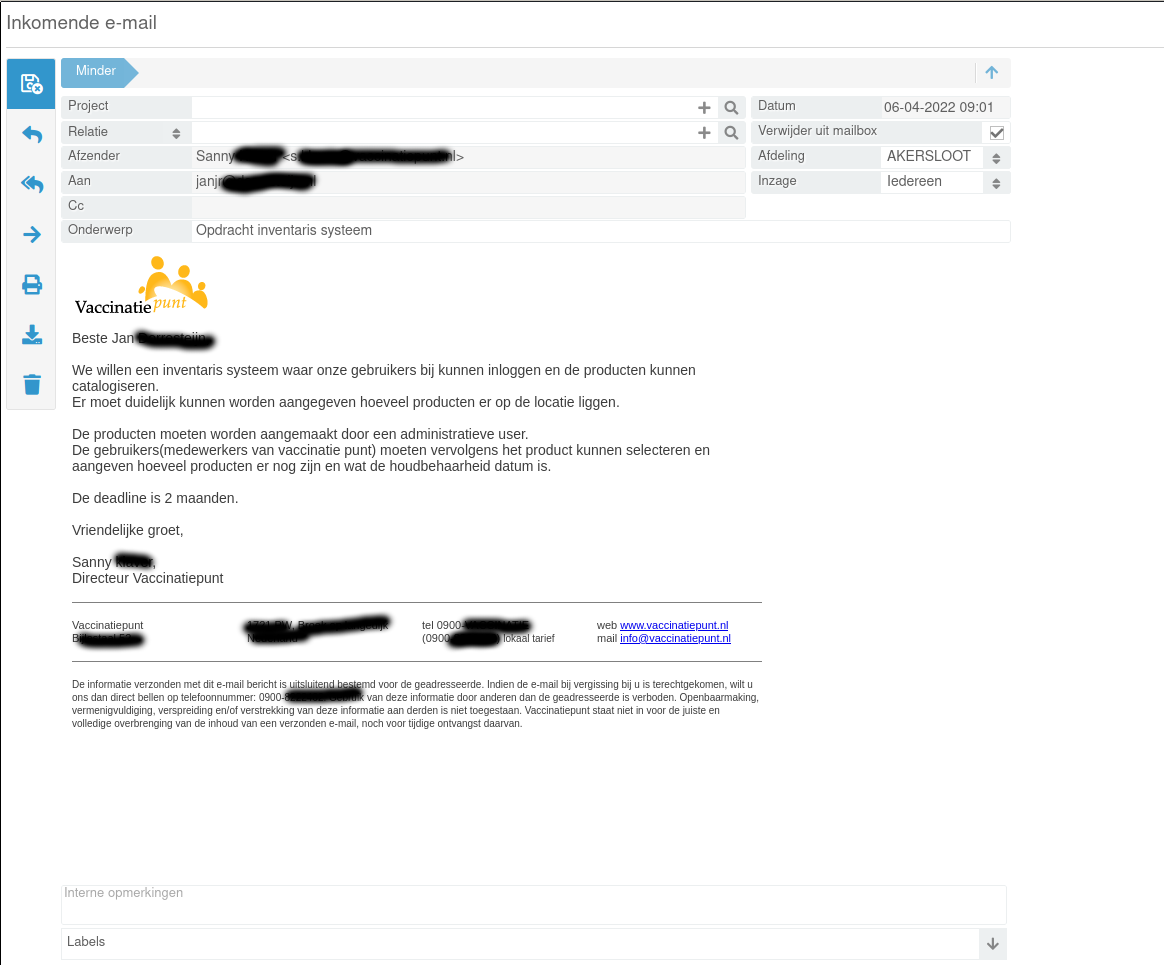
\includegraphics[width=0.95\textwidth]{images/email.png}
			\end{center}
			\caption{email client}
			\label{fig:emailclient}
		\end{figure}
	},
}
